%1095
\newpage
\subsection{例題4-4 色々な絵と文字を表示する}


\begin{description}
    \item \textgt{\bf 考え方}
\end{description}

絵と文字を表示するプログラム(celput.hsp)を改造してみましょう。

\begin{description}
    \item \textgt{\bf \ \ celload “sozai1.jpg”,1}
\end{description}


は「sozai1.jpg」という画像ファイルを表示するための準備をします。

[資料] 背景として使える画面の一例

   ( sozai1.jpg 〜 sozai20.jpg )


\begin{figure}[H]
    \begin{center}
      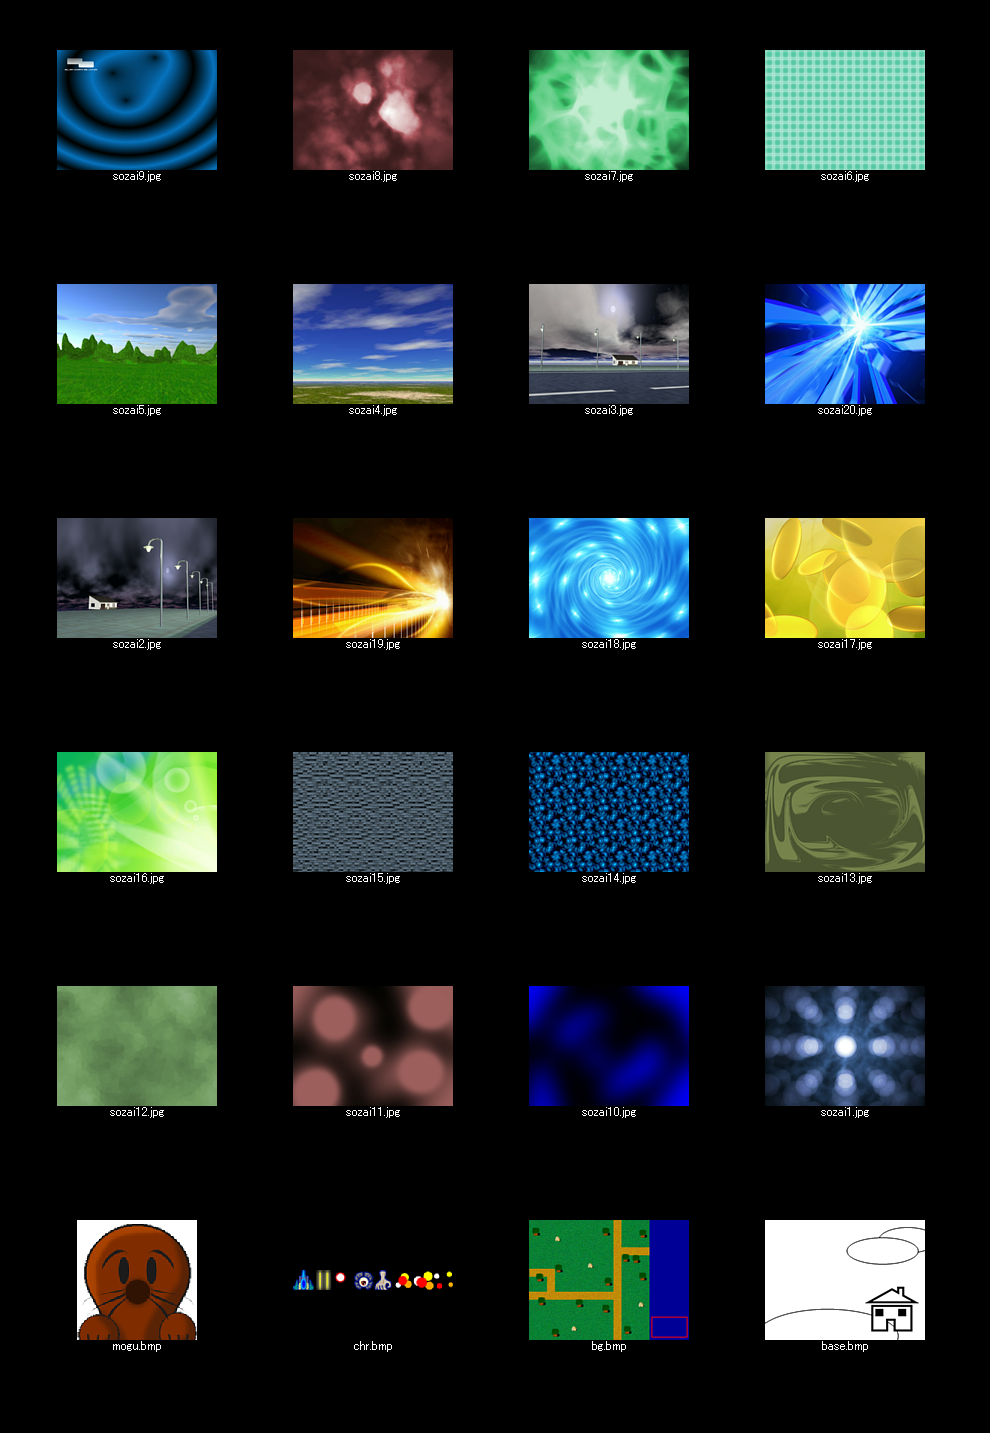
\includegraphics[keepaspectratio,width=14.843cm,height=17.609cm]{text04-img/text04-img014.png}
    \end{center}
    \label{fig:prog_menu}
\end{figure}

試しに、celload命令で指定している画像ファイル名を他のものに変更して、実行してみましょう。

このように自由な絵を使って画面を作っていくことができます。


\begin{description}
    \item \textgt{\bf 例題4-4 答え}
\end{description}



「04」フォルダには、自由に使える素材として「sozai1.jpg」から「sozai20.jpg」まで20種類の画像ファイルが含まれています。

[F5]キーを押して改造した画面がきちんと表示されるかどうか確認しましょう。

mes命令、font命令、color命令、pos命令も書き換えることで、違ったメッセージを表示させることができます。

改造ができたらTAや周りの友達にも見せてあげましょう。

%1158








